\documentclass[12pt, letterpaper]{article}

% Here are some basic userpackages.
\usepackage[utf8]{inputenc}
% \usepackage{graphicx}
% \graphicspath{{images/} }
\usepackage{graphicx}
\usepackage{booktabs}
\usepackage{float}
\graphicspath{{images/Users/sxy/Desktop/A letter.jpg}} % Actually, in Overleaf, it is not necessary to write this command. In real LaTex, we should write this line to upload the file first.
\usepackage{setspace} % setspace: The standard and easiest package for adjusting line spacing.
\usepackage{titlesec} % titlesec: Allows customizing section headings (Optional, for aesthetic purposes).
\usepackage{url} % url: For correct formatting of URLs.
\usepackage[margin=1in]{geometry}
% Set the main font to be LModern (a good default font for modern systems)
\usepackage{lmodern}
% Set section numbering style.

\title{\LaTeX  Learning}
\author{Lisa\thanks{funded by the Overleaf team}}
\date{Oct 2025}
% Here we have preliminarily written the Preamble part, which is something before the main body.


\begin{document} % Together with /enddocument

\maketitle
% This symbol means a comment, it will not be printed out.
\thispagestyle{empty} % Suppress page numbering on the title page
\tableofcontents

\begin{spacing}{1.3}
\section{Basics}
\begin{enumerate}
\item The class refers to the output of the entire document.
\item The preamble defines the document type, input encoding (like UTF-8), and packages.
\end{enumerate}

\subsection{Examples of text form}
% \textbf{} is to bold what you want 
% \textit{} is to italicise what you want
% \underline{} is to underline what you want
% \textsc{} is to print out small capitals
% \texttt{}, used for codes mainly
% \emph{} is to change the form
I love \textbf{linguistics}. -- Bold
\\I love \textit{linguistics}. -- Italic
\\I love \underline{linguistics}. -- Underline
\\\textbf{I love \emph{linguistics}.} -- Change form
\\ System names should be printed out by small capitals, for example \textsc{mood} and \textsc{polartiy}.
\\ \texttt{ "Hello world!"}

\paragraph{However, some packages, such as BEAMER, can change the function of emphasis.}


\subsection{List}
There are two ways under different environments to establish a list. 
\begin{enumerate}
\item Unoredered list or bulleted list: use begin/end itemize
\item Ordered list or numbered list: use begin/end enumerate
\end{enumerate}

\section{Graphics}
\subsection{Add graphics}
\begin{itemize}
    \item Firstly, we should upload a graphic. 
    \item Then we should use the package "graphicx", including "includegraphics" and "graphicspath" as listed below. graphicspath{}
    \item Note that for \textbackslash includegraphics, we should ALWAYS include the file extension (e.g., .jpg or .png).
\end{itemize}
Let us try.
Here is a letter from the great linguist Michael Halliday to Christian Matthiessen:

\begin{figure}[H] % we use another package called "float" to make the figure static in its position.
% H means Here.
    \centering
    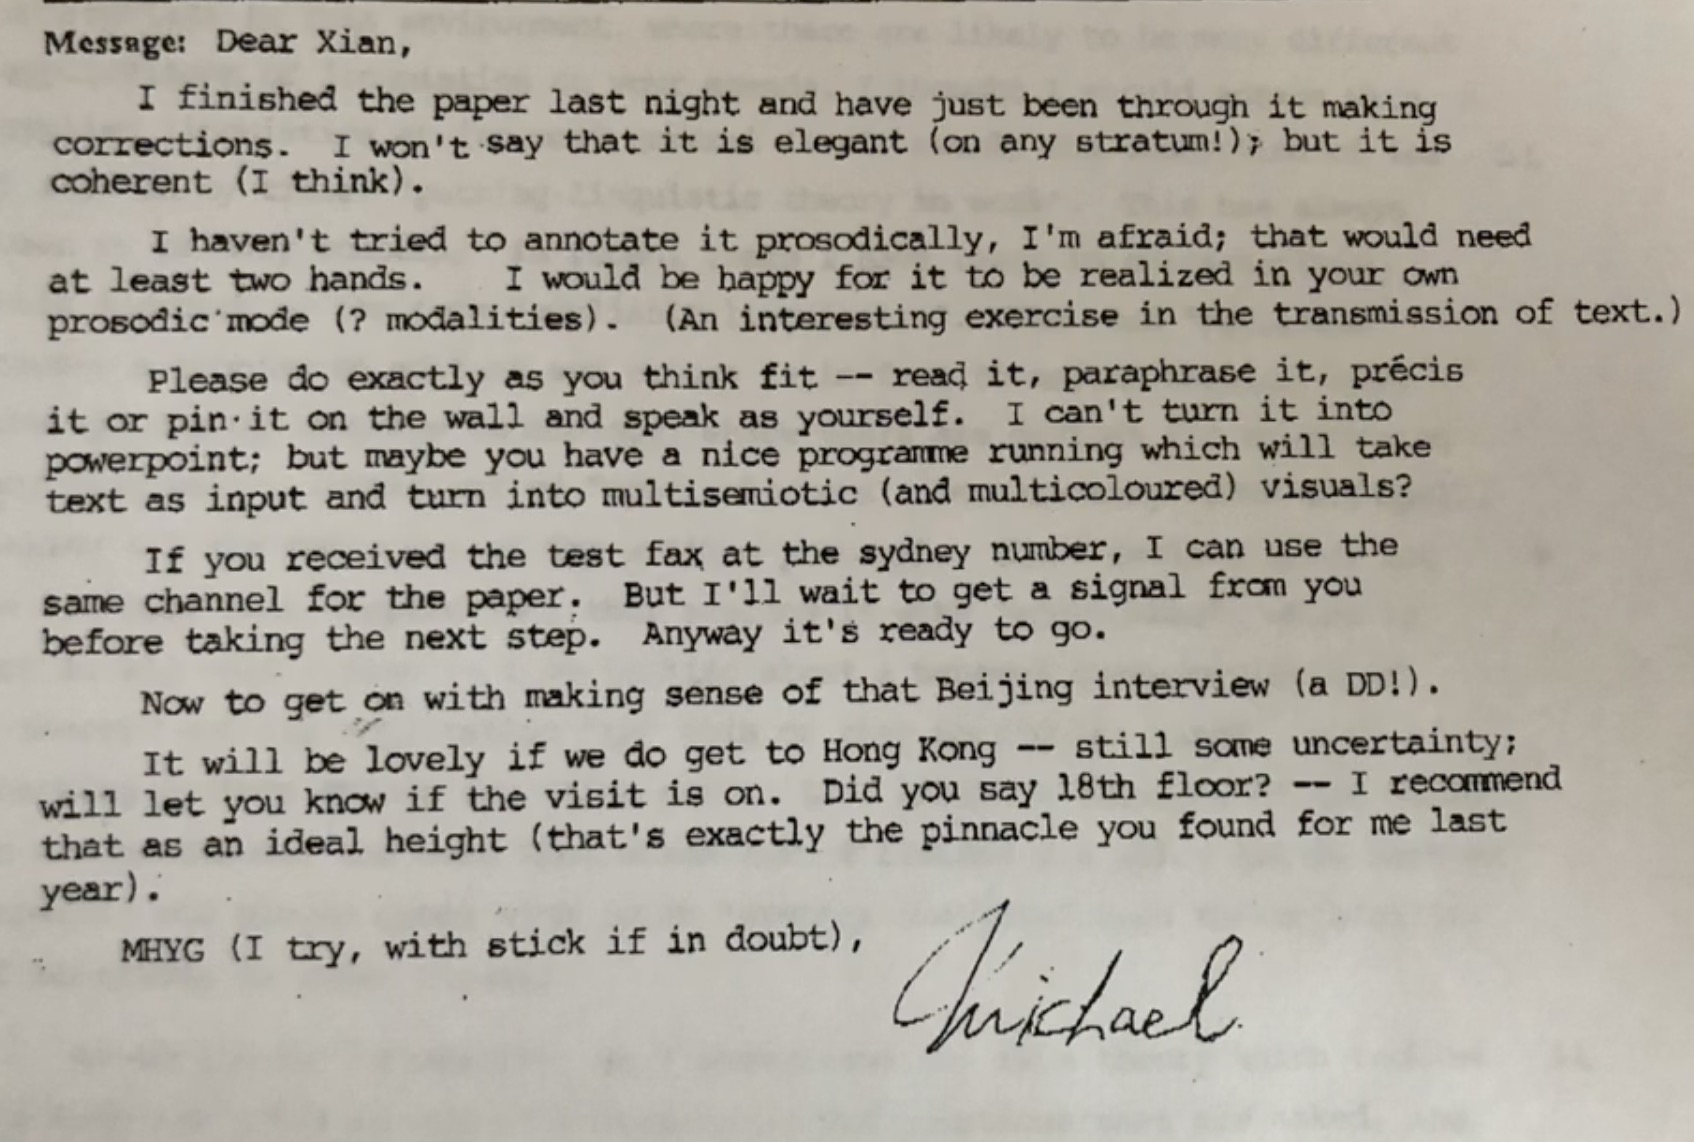
\includegraphics[width=0.5\linewidth]{A letter.jpg}
    \caption{A letter between two linguists}
    \label{fig:mesh1}
\end{figure}


\subsection{Captions, labels and references}
Under the environment of Figure, we can add figure names, tags and references for a picture.
\begin{figure}[H]
    \centering
    
\includegraphics[width=0.5\textwidth]{Memo.jpg}
    \caption{Memorial bench of Halliday}
    \label{fig:mesh2}
\end{figure}

As you can see in the figure \ref{fig:mesh2}, this bench is used in memory of M.A.K Halliday. Also, in the page \pageref{fig:mesh1} is the same example.

Note:
\begin{itemize}
    \item caption{} is to set a label for a figure. (Either above or below the figure is okay.)
    \item label{} when we want to cite this figure, then we use this code
    \item ref{} will be replaced by the number corelated with the figure
\end{itemize}


\section{Mathematics}
\begin{itemize}
    \item We can use sqaure brackets or begin/end math in inline mode.
    \item Or we can use brackets, begin/end displaymath, or begin/end equation in display mode.
    \item Note that EQUATION is from a package called asmath.
\end{itemize}
Let us try.

The mass-energy equivalence is described by the famous equation.

\[E=mc^2 \]

discovered in 1905 by Albert Einstein.

In natural units (c = 1), the formula expresses the identity
\begin{equation}
E=m
\end{equation}

\section{Document settings}
\subsection{List environments}

\subsubsection{Unordered list}
\begin{itemize}
    \item Use \texttt{\textbackslash begin\{itemize\};\textbackslash end\{itemize}
    \item Use \texttt{\string\item} for each item
    \item Suitable for bulleted lists.
\end{itemize}

\subsubsection{Ordered list}
\begin{enumerate}
    \item Use \texttt{\string\begin\{enumerate\}}
    \item Use \texttt{\string\item} for each item
    \item Suitable for automatically numbered lists.
\end{enumerate}


\subsection{Document Structure and Basic Commands}
\subsubsection{Main boday layout}
\begin{enumerate}
    \item How to make an abstract
We will use \textbackslash begin and end abstract before and after the main body of an abstract. Let's see:
\begin{abstract}
This is a simple paragraph at the beginning of the
document. A brief introduction about the main subject.
\end{abstract}

    \item How to start a new paragraph

Double-click "Enter" on keyboard, or use double slashes or newline to create a new line.

Note: that do not use too much newlines to simulate the borderlines between paragraphs.
    \item How to start a new chapter

Here are some basics: \textbackslash part \textbackslash chapter \textbackslash section \textbackslash subsection \textbackslash subsubsection \textbackslash paragraph \textbackslash subparagraph
\end{enumerate}

If we use *, then \LaTeX will stop enumerating sections.

\subsubsection{Line Spacing Control}

LaTeX's default line spacing (known as \textbf{\texttt{linespread}}) is approximately 1.2 times the font size. To adjust it easily and reliably, we use the setspace package, which is the most common standard method.

Here we can see one example:
\begin{spacing}{1.0} % Temporarily set to single for comparison
\paragraph{Single Spacing(\texttt{\string\singlespacing})}

This is the default single spacing.This is the default single spacing.This is the default single spacing.
\end{spacing}
\begin{spacing}{1.5}
\paragraph{1.5 Line Spacing(\texttt{\string\onehalfspacing})}

This is commonly used spacing for many international academic papers and reports. In the \texttt{setspace} package, this command corresponds to a factor of about 1.5.
\end{spacing}
\begin{spacing}{2.0}
\paragraph{Double Spacing (\texttt{\string\doublespacing})}
This is the standard double spacing for most PhD theses and papers requiring review. It provides maximum reading space.
\end{spacing}

\subsubsection{Custom Line Spacing}

If you need a very precise, non-standard line spacing, you can use the \texttt{\string\setstretch\{factor\}} command.

Here is an example to set a custom 1.3 Line Spacing, which means to set stretch to 1.3.
\begin{itemize}
    \item We can use \texttt{\string\setstretch\{1.3\}} to set 1.3 line spacing, which is slightly larger than single spacing.
    \item \textbf{Note:} The \texttt{setspace} package commands automatically add appropriate vertical space between paragraphs.
\begin{spacing}{1.3}
This is an example of custom line spacing set using the \texttt{\string\setstretch\{1.3\}} command. This method is very precise, but note that you may need to fine-tune the factor based on the overall appearance of the document. This paragraph demonstrates the effect of 1.3 line spacing, which falls between single and 1.5 spacing.
\end{spacing}
\end{itemize}

\section{Paragraph Control}
\subsection{Manually Adding Vertical Space}
If you need to add extra space between two paragraphs, you can use:
\begin{itemize}
    \item \texttt{\string\smallskip}: Smaller space.
    \item \texttt{\string\medskip}: Medium space (recommended).
    \item \texttt{\string\bigskip}: Larger space.
    \item \texttt{\string\vspace\{1cm\}}: Specify an arbitrary vertical space, for example, 1 centimeter.
\end{itemize}

\subsection{Controlling Paragraph Indentation}
\LaTeX-defaults to indenting the beginning of every new paragraph, except for the paragraph immediately following a heading.
\begin{enumerate}
    \item Remove indentation: use the \texttt{\string\noindent} command at the start of a paragraph to suppress the current paragraph's indentation.

\noindent \textbf{See this example}:

\noindent This is a paragraph with an indentation removed.

    \item Force indentation: Use the command \texttt{\string\indent} at the beginning of a paragraph to force the current paragraph into indentation.
\end{enumerate}

\subsection{Forcing a Line Break}
\begin{itemize}
    \item New Paragraph: Leave a blank line (two carriage returns). This is the recommended approach.
    \item Force Line Break without Starting New Paragraph: Use \texttt{\string\newline} or \texttt{\string\textbackslash{}\textbackslash{}}.
\end{itemize}
This is one paragraph, and I use \texttt{\string\textbackslash{}\textbackslash{}} \\ to force a line break here, but it remains the same paragraph.


\section{Tables}
\subsection{Creating a table}
Create a table under the environment of tabular.

In this example:
\begin{center}
\begin{tabular}{ c c c }
 cell1 & cell2 & cell3 \\
 cell4 & cell5 & cell6 \\
 cell7 & cell8 & cell9
\end{tabular}
\end{center}

\begin{itemize}
    \item center is used to make everything in central place;
    \item this triplet of c is to show LaTeX that we want a three rows with texts in central place. Another way to realise this method is to use "/r" or "/l".
    \item "\&" is to separate different items, so in each line the number of this symbol is not greater than the number of columns.
\end{itemize}
\subsection{Add borderlines}
Still, we use the same table.
\begin{center}
\begin{tabular}{c c c}
     cell1 & cell2 & cell3 \\
     cell4 & cell5 & cell6 \\ 
     cell7 & cell8 & cell9 \\ 
\end{tabular}
\end{center}

Now we can use the horizontal line command \textbackslash hline and the vertical line parameter | to add borders.

This command (\textbackslash hline) will insert a horizontal line. In this example, we add horizontal lines at the top and bottom of the table. 

There is no limit to the number of times you can use \textbackslash hline.

You can see a second example below.
\begin{center}
\begin{tabular}{|c | c c c|}
\hline
     Name & Text & Int & Exp \\ [0.5ex] % it is used to add height to this line.
\hline\hline % this can be refined as cline{1-4}
     Mary & 15 & 6 & 43 \\
     Beverly & 10 & 4 & 56 \\
\hline
\end{tabular} 
\end{center}

Now, a new table has been generated, listing two mothers' Theme usage in \textit{The Big Bang Theory}, Ep.23, Season 8.

\paragraph{Sometimes, it is quite difficult to make a table in \LaTeX, try out the website "TablesGenerator.com ".}

\subsection{Captions, labels and reference}
This section uses the same principles as Section 2.1... The only difference is that this time the environment is "table", not "figure" anymore.

Here is an example based on the Theme analysis of two mothers. Now we are going to add captions, labels and references.

Table \ref{table:data} is Theme analysis of two mothers.
\begin{table}[h]
\begin{center}
\begin{tabular}{|c | c c c|}
\hline
     Name & Text & Int & Exp \\ 
\toprule
     Mary & 15 & 6 & 43 \\
     Beverly & 10 & 4 & 56 \\
\hline
\end{tabular} 
\end{center}
\caption{Theme analysis}
\label{table:data} %Caption and label should be listed outside the tabular environment.
\end{table}

I have made some mistakes, so here are some notes:

\begin{itemize}
    \item In \LaTeX, the \textbackslash caption and \textbackslash label commands MUST be placed outside the tabular environment but inside the table floating environment.
    \item When using captions, labels and references in \LaTeX, we should compile the document twice for the references to work correctly. In Overleaf, this is handled automatically.
\end{itemize}

\section{Add a Content}
This is easy to operate. We use \textbackslash tableofcontents to make sure every chapters and sections in \textbf{Section 3} can be added in \textbf{Preamble}.

If some unmarked sections are to added, use "\textbackslash addcontentsline".

\end{spacing}
\begin{center}
    \Huge
    \textbf{Thanks! Have fun with coding!}
\end{center}
\end{document}